%%%%%%%%%%%%%%%%%%%%%%%%%%%%%%%%%%%%%%%%%%%%%%%%%%%%%%%%%%%%
%%% LIVECOMS ARTICLE TEMPLATE FOR BEST PRACTICES GUIDE
%%% ADAPTED FROM ELIFE ARTICLE TEMPLATE (8/10/2017)
%%%%%%%%%%%%%%%%%%%%%%%%%%%%%%%%%%%%%%%%%%%%%%%%%%%%%%%%%%%%
%%% PREAMBLE
\documentclass[9pt,bestpractices]{livecoms}
% Use the 'onehalfspacing' option for 1.5 line spacing
% Use the 'doublespacing' option for 2.0 line spacing
% Use the 'lineno' option for adding line numbers.
% Use the 'pubversion' option for adding the citation and publication information to the document footer, when the DOI is assigned and the article is added to a live issue.
% The 'bestpractices' option for indicates that this is a best practices guide.
% Omit the bestpractices option to remove the marking as a LiveCoMS paper.
% Please note that these options may affect formatting.

\usepackage{subcaption}
\usepackage{lipsum} % Required to insert dummy text
\usepackage[version=4]{mhchem}
\usepackage{siunitx}
\DeclareSIUnit\Molar{M}
\usepackage[italic]{mathastext}
\graphicspath{{figures/}}

%%%%%%%%%%%%%%%%%%%%%%%%%%%%%%%%%%%%%%%%%%%%%%%%%%%%%%%%%%%%
%%% IMPORTANT USER CONFIGURATION
%%%%%%%%%%%%%%%%%%%%%%%%%%%%%%%%%%%%%%%%%%%%%%%%%%%%%%%%%%%%

\newcommand{\versionnumber}{0.2}  % you should update the minor version number in preprints and major version number of submissions.
% Do not add a newline in the next command, no matter how long the repository name is, as it will break the link in the PDF.
\newcommand{\githubrepository}{\url{https://github.com/stepan-srsen/ML_NAMD_best_practices_paper}}  %this should be the main github repository for this article.

%%%%%%%%%%%%%%%%%%%%%%%%%%%%%%%%%%%%%%%%%%%%%%%%%%%%%%%%%%%%
%%% ARTICLE SETUP
%%%%%%%%%%%%%%%%%%%%%%%%%%%%%%%%%%%%%%%%%%%%%%%%%%%%%%%%%%%%
\title{Data-driven insights and best practices on machine learning nonadiabatic dynamics simulations [Article v\versionnumber]}


% \author[1*]{Firstname Middlename Surname}
% \author[1,2\authfn{3}]{Firstname Middlename Familyname}
% \author[2\authfn{4}]{Firstname Initials Surname}
% \author[2*]{Firstname Surname}

\author[1]{Carolin Müller}
\author[2,3]{Brigitta Bachmair}
\author[4]{Rachel Crespo-Otero}
\author[5]{Jingbai Li}
\author[3,6]{Sascha Mausenberger}
\author[7]{Max Pinheiro Jr}
\author[6,8]{Štěpán Sršeň}
\author[4]{Graham Worth}
\author[9*]{Steven A. Lopez}
\author[10,11*]{Julia Westermayr}

% \affil[1]{Institution 1}
% \affil[2]{Institution 2}

% \affil[1]{Physics and Materials Science Research Unit, University of Luxembourg, 1511 Luxembourg, Luxembourg}
\affil[1]{Computer Chemistry Center, Friedrich-Alexander University of Erlangen-Nuremberg, Nägelsbachstraße, 91052 Erlangen, Germany}
\affil[2]{Research Platform on Accelerating Photoreaction Discovery (ViRAPID), University of Vienna, 1090 Vienna, Austria}
\affil[3]{Vienna Doctoral School in Chemistry (DoSChem), University of Vienna, Währinger Straße 42, 1090 Vienna, Austria}
\affil[4]{Department of Chemistry, University College London, 20 Gordon Street, London, WC1H 0AJ, UK}
\affil[5]{Hoffmann Institute of Advanced Materials, Shenzhen Polytechnic University, 7098 Liuxian Boulevard, Shenzhen, Guangdong 518055, P. R. China}
\affil[6]{Institute of Theoretical Chemistry, Faculty of Chemistry, University of Vienna, Währinger Str. 17, 1090 Wien, Austria}
\affil[7]{Aix Marseille University, CNRS, ICR, Marseille, France}
\affil[8]{Department of Physical Chemistry, University of Chemistry and Technology, Technická 5, 162 28 Prague, Czech Republic}
\affil[9]{Department of Chemistry \& Chemical Biology, Northeastern University, 805 Columbus Avenue, Boston, MA, 02120 USA}
\affil[10]{Faculty of Chemistry and Mineralogy, University of Leipzig, Johannisallee 29, 04103 Leipzig, Germany}
\affil[11]{Center for Scalable Data Analytics and Artificial Intelligence (ScaDS.AI), Dresden/Leipzig,
Germany}

\corr{s.lopez@northeastern.edu}{SAL}  % Correspondence emails.  FMS and FS are the appropriate authors initials.
\corr{julia.westermayr@uni-leipzig.de}{JW}

\orcid{Carolin Müller}{0000-0002-5968-2216}
\orcid{Brigitta Bachmair}{0000-0002-2346-7995}
\orcid{Rachel Crespo-Otero}{0000-0002-8725-5350}
\orcid{Jingbai Li}{0000-0003-4743-0318}
\orcid{Sascha Mausenberger}{0009-0003-8136-8770}
\orcid{Max Pinheiro Jr}{0000-0002-5120-4172}
\orcid{Štěpán Sršeň}{0000-0001-7723-4540}
\orcid{Graham Worth}{0000-0002-2044-4499}
\orcid{Steven A. Lopez}{0000-0002-8418-3638}
\orcid{Julia Westermayr}{0000-0002-6531-0742}

% \contrib[\authfn{1}]{These authors contributed equally to this work}
% \contrib[\authfn{2}]{These authors also contributed equally to this work}

% \presentadd[\authfn{3}]{Department, Institute, Country}
% \presentadd[\authfn{4}]{Department, Institute, Country}

\blurb{This LiveCoMS document is maintained online on GitHub at \githubrepository; to provide feedback, suggestions, or help improve it, please visit the GitHub repository and participate via the issue tracker.}

%%%%%%%%%%%%%%%%%%%%%%%%%%%%%%%%%%%%%%%%%%%%%%%%%%%%%%%%%%%%
%%% PUBLICATION INFORMATION
%%% Fill out these parameters when available
%%% These are used when the "pubversion" option is invoked
%%%%%%%%%%%%%%%%%%%%%%%%%%%%%%%%%%%%%%%%%%%%%%%%%%%%%%%%%%%%
\pubDOI{10.XXXX/YYYYYYY}
\pubvolume{<volume>}
\pubissue{<issue>}
\pubyear{<year>}
\articlenum{<number>}
\datereceived{Day Month Year}
\dateaccepted{Day Month Year}

%%%%%%%%%%%%%%%%%%%%%%%%%%%%%%%%%%%%%%%%%%%%%%%%%%%%%%%%%%%%
%%% ARTICLE START
%%%%%%%%%%%%%%%%%%%%%%%%%%%%%%%%%%%%%%%%%%%%%%%%%%%%%%%%%%%%

\begin{document}

\begin{frontmatter}
\maketitle

\begin{abstract}
Exploring molecular excited states holds immense significance across organic chemistry, chemical biology, and materials science and understanding the photophysical properties of molecular chromophores is crucial for designing nature-inspired functional molecules, with applications ranging from photosynthesis to pharmaceuticals.
Nonadiabatic molecular dynamics simulations are powerful to investigate the photochemistry of molecules and materials, but demand extensive computing resources, especially for complex molecules and environments. To address these challenges, the integration of machine learning has emerged. Machine learning algorithms can be used to analyze vast datasets and accelerate discoveries by identifying relationships between geometrical features and ground and excited-state properties. However, challenges persist, including acquiring accurate excited-state data and managing the complexity of the data. This article provides an overview of recent and best practices in machine learning for nonadiabatic molecular dynamics, focusing on pre-processing, surface fitting, and post-processing of data.
\end{abstract}

\end{frontmatter}




\section{Introduction}

A deeper understanding of molecular excited states holds profound significance across organic chemistry, chemical biology, and materials science. Understanding the role of photophysical properties of molecular chromophores and subsequent photodynamics is needed to design molecules with nature-inspired functions (e.g., photosynthesis and vision). Molecular discoveries can be scaled up to the materials level, encompassing light-harvesting molecules, catalysts, or even drugs that act through photochemical reactions. Beyond fundamental insights in photochemistry, there is a high likelihood of broader impacts in atmospheric chemistry, solar energy conversion, photoresponsive materials, and molecular electronics.

Nonadiabatic molecular dynamics (NAMD) simulations are increasingly used to unravel structure-property relationships by resolving sub-nanosecond photodynamics simulations and guiding the design of novel chromophores, materials, and devices.  NAMD simulations consider nonadiabatic effects beyond the Born-Oppenheimer approximation, arising from the interactions between excited states driven by their couplings with molecular vibrations. Substantial computing power is required to identify the real-time excited-state molecular vibrations and reaction pathways toward all possible photoproducts. Mixed quantum-classical (MQC) molecular dynamics methods are acceptable because they compromise computational efficiency and accuracy due to the Born-Oppenheimer approximation \cite{RN90}. This approximation propagates quantum mechanical (QM) electrons and classical nuclei. However, popular density functional theory (DFT) fails when describing the electronic structure of strongly correlated systems (e.g., some organometallic complexes, Rydberg, charge-transfer-states, and geometries near conical intersections). Multiconfigurational methods (MC) can overcome these limitations but are more computationally expensive and require additional expertise (e.g., active space selection). These factors are compounded in NAMD because of the thousands of requisite and sequential excited-state calculations. The computational demands of such investigations become even more challenging in large molecules and complex environments (e.g., explicit solvation), slowing progress in numerous scientific applications \cite{RN89}. This challenge has spurred the integration of machine learning (ML) techniques into studying photodynamics to overcome existing limitations and unlock new possibilities \cite{RN131,RN98,RN121,RN129}.

ML algorithms leverage vast datasets of QM calculations or experimental measurements to discern patterns and correlations \cite{RN129, RN101, RN116, RN150}. ML models learn from these data to identify intricate relationships between ground and excited-state molecular structures and their energies, forces, and nonadiabatic couplings. Their computational efficiency, compared to QM calculations, accelerates discoveries. The field of ML-photodynamics is highly dynamic yet still in its infancy. Several substantial challenges remain to realize its full potential: 1)  difficulty in attaining excited state data, 2) the arbitrary phase of the wavefunction and corresponding complexity of the non-unique definition of excited-state properties, and 3) discontinuities near regions of solid coupling \cite{RN98, RN105}. These challenges are technically difficult, and the computational costs have slowed the influx of new researchers to enter this new field. Therefore, we provide an overview of the current state of the art of ML in NAMD simulations and offer a view of best practices in this field that might be established in future research of ML models. The work is structured into three sections, focusing on pre-processing of data, surface fitting, and post-processing of ML-generated data.

% \section{Prerequisites}

% Here you would identify prerequisites/background knowledge that are assumed by your work and your checklist which you view as critical, ideally giving links to good sources on these topics.
% Checklists are normally focused on errors made by users with training and experience in molecular simulations, so you can assume a basic familiarity with the fundamentals of molecular simulations.

% \section{Rationale}

% Your Rationale section, or sections, can follow or precede your checklist (we expect that often, following the checklist will be preferable) and provide the necessary rationale for the checklist, and act as more complete \emph{best practices} description.
% This should include 1) significant detail as to the possible alternative ways to accomplish a given task, 2) description of advantages and disadvantages of the various approaches, and 3) significant literature documentation about reasons for choices.

% \subsection{Algorithms and Pseudocode}
% \label{sec:reference_this}

\section{Pre-processing}
\label{sec:preprocessing}

Understanding spectroscopic features and photochemical reaction outcomes is critically important because atomistic resolution of molecular excited state structures is not yet possible with experiments. The distinct electronic structures of molecules in their ground and excited states provide a challenge that can be overcome with QM calculations in close collaboration with experimental techniques \cite{RN107}. ML has emerged as a revolutionary force in computational chemistry to accelerate MQC calculations, enabling excited-state photodynamics simulations for medium-sized molecules on pico- to nanosecond time scales \cite{RN140, RN132}.

This section will discuss the best practices for generating training data ready for ML models (i.e., from available QM trajectories). We first provide an overview of common QM methods to obtain the trajectories' energies, forces, and couplings and explain the data types suitable for training ML models. The second part discusses preprocessing techniques to convert trajectory data into ML-learnable data.

\subsection{Introduction to NAMD Simulations}

NAMD methods have evolved into various approaches, from quantum to semiclassical methods. Quantum methods, such as Multiconfiguration time-dependent Hartree  (MCTDH) \cite{RN87} or variational multiconfigurational Gaussian (vMCG) \cite{RN88} propagation methods, directly consider the nuclear wavefunctions and offer insights into nuclear quantum effects. An example of wavefunction propagation is shown in Figure \ref{fig:NAMD}a, where a wavepacket is split along the trajectory. However, because of their computational costs, these methods usually require selecting a few degrees of freedom for the propagation, the assumption of model potential energy surfaces (PESs) and the use of linear vibronic coupling models. Trajectory-based methods, such as ab initio multiple spawning (AIMS) \cite{RN118, RN85, RN86}, Ehrenfest dynamics \cite{RN141, RN154}, and trajectory surface hopping \cite{RN154, RN133, RN134}, assume that the nuclear wave function can be approximated by a swarm of classical trajectories, exemplified in Figure \ref{fig:NAMD}b. Among these approaches, the trajectory surface hopping method is one of the most widely used techniques for investigating photoinduced processes and reactions of medium-sized molecules on the picosecond timescale \cite{RN118}.

Trajectory surface hopping simulations are usually performed on the fly, considering all vibrational degrees of freedom. However, approximated PESs obtained from, for instance, the linear vibronic coupling model, could also be used \cite{RN3}. Notably, model PESs make the simulations much more computationally efficient but introduce approximations. Accurate solutions for linear vibronic coupling systems can only be obtained for rigid systems. ML-based PESs offer higher accuracy and high computational efficiency by learning quantum chemical reference data \cite{RN98, RN139}. We will thus focus on surface hopping trajectory data that can be fed into ML models, facilitating NAMD simulations.

\begin{figure}[hbt!]
\centering
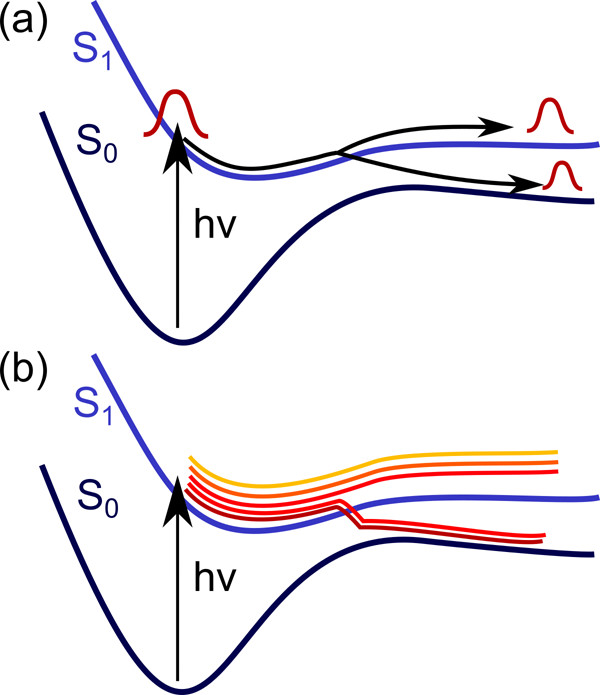
\includegraphics[width=0.9\linewidth]{figures/NAMD_JW2020.jpeg}
\caption{a) Quantum and b) classical propagation of the nuclei in excited-state molecular dynamics simulations. It is reproduced from ref. \cite{RN98} under CC-BY 4.0.}
\label{fig:NAMD}
% \figdata{This is a description of a data source.}
\end{figure}

\subsubsection{Surface hopping methods}
\label{sec:surfacehop}

Surface hopping methodologies assume that the nuclei move on a single PES. They undergo nonadiabatic transitions between electronic states instantaneously and span relatively small regions of the configuration space. The nonadiabatic transitions are approximated with instantaneous switches between adiabatic PESs, giving rise to "surface hopping." The mixed quantum-classical nature of surface hopping methods offers favorable simplicity, efficiency, and scalability for studying nonadiabatic phenomena in molecular systems. An example with a swarm of 5 trajectories, where two undergo a transition from the excited state to the ground state, is shown in Figure \ref{fig:NAMD}b.

Several NAMD packages are available to generate the surface hopping trajectories, to name a few: SHARC \cite{RN139}, Newton-X \cite{RN157, RN2}, PyRAI$^2$MD \cite{RN140}, and JADE-NAMD \cite{RN84}. Despite the various implementations of the surface hopping methods in these packages, they share the same aspects to produce the trajectory data, including the surface hopping algorithms, excited-state calculations, and generation of initial conditions, often used as starting structures for NAMD.

The wave function in surface hopping is a linear combination of multiple electronic states with the same or different spin multiplicities at specific nuclear positions. The temporal evolution of nuclear positions, referred to as trajectory propagation, updates the nuclear coordinates and velocities by integrating Newton's equation of motion (i.e., classical nuclear motion). The coefficients of the electronic states determine the current state for propagating the nuclear trajectory. The square of these coefficients represents the electronic state populations, and their time derivatives indicate the tendency of nonadiabatic electronic transitions between states \cite{RN118}.

The fewest switches surface hopping (FSSH) method assumes the least number of switches between two electronic states, meaning that electronic population transfer occurs primarily from one electronic state to another. The transition probabilities in fewest switches surface hopping dynamics depend on the nonadiabatic couplings (NACs) between electronic states with the same spin multiplicity (i.e., internal conversion) \cite{RN83}, which describe the steepest changes in the wave function as nuclear motions occur. When intersystem crossing is considered, spin-orbit couplings (SOCs) are also required to account for hops between electronic states with different spin multiplicities (i.e., intersystem crossing) \cite{RN82, RN81}. The NACs and SOCs connect the classical nuclear dynamics and electronic wave function, governing the temporal evolution of electronic populations over all considered states.

It is important to note that the NACs contain a phase factor dependent on the phases of the wavefunction of the coupled electronic states. Since the wavefunction phase is randomly initialized at different nuclear positions, one must correct the couplings to ensure the same phase for dynamics. The phase correction of couplings is often performed by computing their overlap between two structures at adjacent time steps \cite{RN132, RN113}. These complexities require additional steps for rigorous data preprocessing for ML, which we will further discuss in section \ref{sec:couplings}. In addition, traditional FSSH may show overcoherence between electronic states because the population transferred to an upper or lower state follows the gradients of the current state. Various approaches have been developed to address overcoherence, including augmented FSSH (A-FSSH), decoherence-induced surface hopping (DISH), methods based on the decay of mixing (DM), and overlap decoherence correction (ODC), among others. All these methods could be used to generate training data for ML. However, due to its simplicity and effectiveness, the most commonly used approach is based on the simplified decay of mixing, which corrects the coefficients at each time step. Overcoherence is usually accounted for in many NAMD programs by applying approximations, such as the ones proposed by Persico and Granucci \cite{RN139, RN157, RN83, RN125}.

Some quantum chemical software can compute NACs; the so-called Baeck-An approximation \cite{RN79, RN80} is one approximation from which various formulas have been derived. For instance, Westermayr et al. used the Hessian of the squared energy gap potential and the gradient difference vectors, defining the branching space, to approximate NACs using ML \cite{RN103, RN104, RN78}. Baeck-An couplings, however, are only accurate in regions of the configuration space where two PESs are nearly degenerate. Thus, it is suggested to set the couplings to 0 when two PESs have a $\Delta E>0.5$ eV \cite{RN81, RN113}. Alternatively, the Landau-Zener scheme can be used to compute hopping probabilities; Landau-Zener requires the evaluation of the energy gaps and their time derivatives, obtained by finite differences along the trajectories, and applies to intersystem crossing. The results from nonadiabatic dynamics with Landau-Zener agree well for small to medium organic systems \cite{RN77}. A similar approach relying only on the PES shape is the Zhu-Nakamura theory of surface hopping \cite{RN76}, which uses energies and gradients of two crossing states for the hopping probability calculations. The forces are diabatized in a generalized 1D model based on three-point interpolation \cite{RN75}. This method agrees well with the fewest switches surface hopping and applies to intersystem crossing \cite{RN75, RN74, RN73, RN72}. Because of the assumption of a particular topology of the PES for the electron transitions, the results obtained with these can be compared with either FSSH, quantum dynamics and or experimental information.  

\subsubsection{Electronic structure methods for excited states}
\label{sec:elstructure}

When performing NAMD simulations, selecting a quantum chemical reference method is one of the most critical steps, as it determines the quality of the dynamics along several PESs \cite{RN105, RN99}. For example, the NAMD simulations of H-adenine showed diverging outcomes depending on the quantum chemical reference method used \cite{RN71}. Unfortunately, MC methods, such as complete active space self-consistent field (CASSCF) \cite{RN138} or its second order perturbation theory (PT2) extension, CASPT2 \cite{RN70}, are often computationally prohibitive. Therefore, alternative data-driven approaches (e.g., $\Delta$ML \cite{RN112}) or transfer learning \cite{RN69} between two different quantum chemical methods should be considered. 

Single configurational (SC) methods compute excited-state electronic structures using the ground state as a reference under the adiabatic approximation, such as time-dependent density functional theory (TDDFT) \cite{RN143}, approximate second-order coupled-cluster (CC2) \cite{RN68}, and algebraic diagrammatic construction to the nth-order (ADC(n)) \cite{RN128}. TDDFT and ADC(2), including their variants, e.g., spin-flip methods \cite{RN62, RN115, RN61}, are the most frequently used SC approaches for trajectory surface hopping (TSH) dynamics simulations \cite{RN67, RN66}. In contrast, the TSH dynamics with CC2 are often not numerically stable \cite{RN71}. TDDFT results are highly dependent on the choice of the functional. Range-separated functionals are known to describe charge transfer states properly. Tuning the range-separation parameter can affect the outcome of the simulations \cite{RN67}. There are several approaches based on ADC(n) including ADC(2), ADC(3), ADC(2)-x, SOS-ADC(2)-x, CVS-ADC(2). The most commonly used method for TSH dynamics is ADC(2), where excitation operators derive the excited states on the ground-state reference from the Møller–Plesset second-order perturbation theory (MP2). The SC methods must be used with care. In TSH dynamics they often fail to describe correct conical intersections between the ground- and the excited state \cite{RN65, RN64}. These two problems are often encountered in computing photochemical reaction pathways, where the reaction could involve doubly excited states and proceed through S$_1$/S$_0$ crossing regions. As such, the common practice to propagate the TSH trajectories with SC methods is to stop the dynamics or assume an instant hopping to the ground state when a crossing region is found, typically when two states are <0.1 eV apart. The instant hopping assumption must be used cautiously because the decay rates might be significantly overestimated \cite{RN63}. On the other hand, the spin-flip technique (e.g., SF-TDDFT) \cite{RN62, RN61} was introduced to restore correct PESs surrounding conical intersections. However, simulations with SF-TDDFT are highly affected by spin-contamination and dynamics simulations, and spin-contamination should be followed along the simulations. Other methods, such as the mixed reference spin-flip TDDFT (MRSF-TDDFT) \cite{RN60} and spin-restricted ensemble-referenced Kohn–Sham (REKS) \cite{RN59} can compute conical intersection at the cost of SC methods. MRSF-TDDFT corrects the issue with SC in SF-TDDFT and has also been used for nonadiabatic dynamics simulations with FSSH \cite{RN58}.

Multiconfigurational methods are essential for accurately describing the molecular electronic structure at degeneracy regions and conical intersections. The MC methods often use the multiconfigurational reference generated by CASSCF. The CASSCF wavefunction requires the so-called active space, which treats the subset of electrons and molecular orbitals with full configurational interaction that addresses the issues of SC methods. The complete active space second-order perturbation theory (CASPT2) \cite{RN70}, n-electron valence state perturbation theory (NEVPT2) \cite{RN1}, and multireference configuration interaction (MRCI) \cite{RN117, RN56, RN57} are two popular MC methods, where CASPT2 directly adds second-order perturbative corrections (i.e., dynamical correlation) to the CASSCF reference. Moreover, the extended multistate (XMS) \cite{RN55}, dynamically weighted (XDW) \cite{RN54}, and rotated multistate (RMS) \cite{RN53} variants of CASPT2 improve the energy corrections near the state-crossing regions. However, the MC methods cannot be used as black-box methods, and running these calculations is limited due to the need for selecting active spaces capable of describing all steps in the dynamics. Intruder states can enter the active space, affecting energy conservation. These issues make excited-state dynamics with MC calculations extremely challenging. Moreover, modern QM programs to do MC calculations only support a limited active space size of 22 electrons and 22 orbitals due to the rapid growth of the hardware requirements. Recent works show that the adaptive sampling configuration interaction (ASCI) method can expand the active space size beyond 50 electrons and 50 orbitals \cite{RN51, RN52}. The costs of MC calculations are only affordable for propagating TSH trajectories of small molecules \cite{RN50, RN49}. Therefore, the CASSCF calculations are commonly used for medium-sized molecules \cite{RN48, RN47, RN46} with careful validations in the excited-state PESs and the photochemical reaction pathway against the MC results. The multiconfiguration pair-density functional theory (MCPDFT) combines CASSCF for static correlations and DFT for dynamical correlations \cite{RN45, RN44}. It shows comparable accuracy to the CASPT2 method at the cost of CASSCF calculations, which offers another choice for obtaining TSH trajectory data \cite{RN43}. In some cases, neither SC nor MC methods can propagate the TSH trajectories correctly, where a combination of QM methods has to be employed \cite{RN104, RN124}.

\subsubsection{Initial conditions}
\label{sec:initcond}

The generation of the initial conditions is one important step for generating starting geometries for TSH trajectories. In addition to providing a set of positions and momenta, the initial conditions should be able to capture some quantum effects in semiclassical simulations.  Most TSH dynamics simulations simulate ultrashort pulses and assume the molecules are vertically excited without explicitly considering the effect of the interaction with the laser \cite{RN42}. The nuclear ensemble approach (NEA) is commonly used for the generation of initial conditions, where a distribution of ground state geometries is used to generate the excited state ensemble \cite{RN152, Srsen2020}. The geometries are usually obtained by Wigner sampling or molecular dynamics (MD) simulations. The Wigner function depends on the vibrational wavefunctions in the position and momentum representations for a set of uncoupled oscillators obtained from a ground-state frequency calculation of the Franck-Condon geometry. The main limitation of these models is the misrepresentation of soft modes (< 500 cm$^{-1}$), which are typically anharmonic. The initial conditions sampled with classical MD simulate a room-temperature Boltzmann-like distribution of the NEA. It corresponds to the effect of an ultrashort light pulse treated in the so-called ‘classical’ limit of an instantaneous optical transition in the Condon approximation. The classical MD sampling of initial conditions was commonly used to investigate the TSH dynamics in biological systems such as rhodopsin \cite{RN48}. Sampling with classical MD produces ensembles with average total energies below the zero point vibrational energy (ZPVE). One solution is to propagate the dynamics at higher temperatures or use the quantum thermostat, where the classical distribution is widened to match the classical distributions \cite{Ceriotti2010, RN42}. Another way to incorporate nuclear quantum effects is via path integral methods \cite{RN110, RN108, Ceriotti2011}. When dealing with molecules that can occur in different conformers, they should be weighted according to a Boltzmann distribution and generate initial conditions based on every available conformer \cite{RN104}.

\subsection{Preprocessing of surface hopping trajectory data}

TSH trajectories record comprehensive time-dependent information of molecules during the NAMD simulations, such as the nuclear coordinates, velocities, electronic state populations, energies, gradients, and interstate couplings. We introduce the data types that ML could extract and discuss the strategies to convert them into machine-learnable representations.

\subsubsection{Choosing trajectory data for machine learning}
\label{sec:trajdatachoice}

A typical TSH dynamics experiment requires 100-500 trajectories to compare to experimental results. Generating training data from TSH dynamics requires careful selections of the molecular structures and the associated ground- and excited-state properties. Selecting trajectory snapshots with a fixed time interval usually gives adequate conformational information for learning ground and excited state PESs. However, the TSH dynamics involve unevenly distributed gaps between the crossing states, and the surface hopping events often happen at the small energy gaps. Thus, the even sampling approach might be insufficient for collecting the surface hopping information; one also needs to sample structures near degeneracy regions.

\subsubsection{Energy and Gradients}
\label{sec:energyandgradients}

The energies and gradients are the most important data to train an ML potential. The TSH trajectories usually contain energy data for each included electronic state, as they can be computed in one single-point calculation. Most FSSH programs only compute the gradients of the “current” populated state needed for propagating the trajectories. In this case, the gradient data only contain partial information about the excited and ground state before and after the surface hopping. On the other hand, one can compute the incomplete gradient data for the selected structures of the TSH trajectories.

We should note that the energy data are a series of scalar values. In contrast, the gradient data are vectorial data stored in 2D arrays of $N$ nuclei and 3 Cartesian coordinates or flattened 1D arrays of $3N$ values. Fitting the energy data is straightforward as they are unique for each molecular structure. However, the gradient data are rotationally covariant (i.e., depending on the molecular orientation). The ML model outputs are scalar values that do not satisfy the rotational covariance, which cannot fit the gradient data. Instead, gradient data is commonly learned as the derivative of the ML potential and the energy. Recent developments in equivariant representations also allow for directly fitting gradients and vectorial properties \cite{RN127, RN95, Schutt21}.

\subsubsection{Interstate couplings}
\label{sec:couplings}

NACs and SOCs are two types of interstate coupling data in TSH trajectories. The availability of NAC data depends on the QM methods. We focus on the TSH trajectories that require explicit NACs. When NACs are unavailable, ML models are trained to predict the energies and gradients and use TSH algorithms without NACs. Preprocessing NAC data is challenging because the random phase of NACs results in discontinuous data as a function of molecular structure. In a TSH dynamics simulation, the NACs can be corrected based on the overlap in two continuous individual timesteps \cite{RN132}. However, the preprocessing of NAC data for ML requires the NACs in all trajectories in the same phase. Thus, additional phase corrections are needed to allow ML models to deal with double-valued properties \cite{RN103, RN41}, which are discussed in detail in the next chapter. 

\section{Surface fitting}
\label{sec:fitting}

Representations of the manifold of potential surfaces and couplings are needed for accurate photodynamical simulations. While many of the problems involved are the same as for fitting ground-state properties, excited states introduce new problems that need to be considered and are discussed here. Fitting the data requires sampling essential regions of configuration space as a function of coordinates. While obtaining the requisite gradients numerically from a potential function is possible, these quantities should be fit directly.

Surface hopping simulations using TSH require couplings in addition to the energies and gradients. These couplings may be NACs or SOCs, depending on the states involved. Not all methods can provide derivative couplings, but approximate couplings can be calculated in many cases.  Some surface hopping methods do not need couplings (e.g., Landau-Zener) \cite{RN77}.

Fitting the couplings can be difficult as the presence of conical intersections leads to singularities and discontinuities, as can be seen in an example in Figure \ref{fig:couplings}. As such, it is better to fit NAC vectors rather than the derivative couplings, as the latter contains the 1/$\Delta E$ term. This can be used to compute “smooth” couplings \cite{RN103} that can be better learned with ML algorithms, as exemplified in Figure \ref{fig:couplings} (blueish dashed line). The couplings also include a random phase that results in sign changes that must be corrected or accounted for.

\begin{figure}[hbt!]
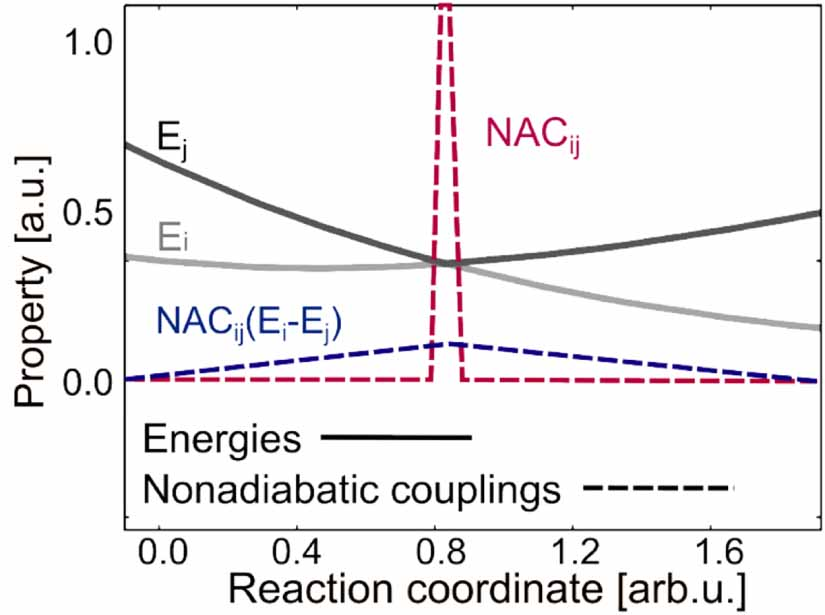
\includegraphics[width=\linewidth]{figures/Couplings_JW2020b.jpg}
\caption{Conical intersection between two states and corresponding nonadiabatic couplings (reddish, dashed lines) including smooth couplings multiplied by the energy gap (blueish, dashed lines). Reproduced from ref. \cite{RN102} under CC-BY 4.0.}
\label{fig:couplings}
% \figdata{This is a description of a data source.}
\end{figure}

If wavepacket propagations are to be performed, surfaces and couplings in a diabatic representation are required rather than the adiabatic representation provided by standard quantum chemistry programs. Relatively smooth diabatic surfaces are more easily fit than adiabatic surfaces; however, there are no general procedures for obtaining suitable data.  Some quantum chemistry codes, such as Molpro, can provide quasi-diabatic energies. The Quantics package can also deliver diabatic energies and couplings using propagation diabatization \cite{RN40}.

\subsection{Machine learning models}

The first choice when it comes to fitting potential energy surfaces and related properties is the selection of the ML model. Two basic classes of ML regression models are currently omnipresent: neural networks (NNs) and kernel methods (KMs) such as kernel ridge regression (KRR), gaussian processes (GP), or support vector machines (SVM. The choice depends on the size of the ensemble of nuclear geometries \cite{RN102, RN39}. While KMs are relatively efficient with small datasets, they suffer from poor scaling ($N^3$ with $N$ being the number of samples). Using KMs for <2000 data points is usually more efficient, while NNs are more appropriate for larger samples. A classification of frequently used ML algorithms and descriptors is shown in Figure \ref{fig:potentials} \cite{RN39}.

\begin{figure*}[hbt!]
\centering
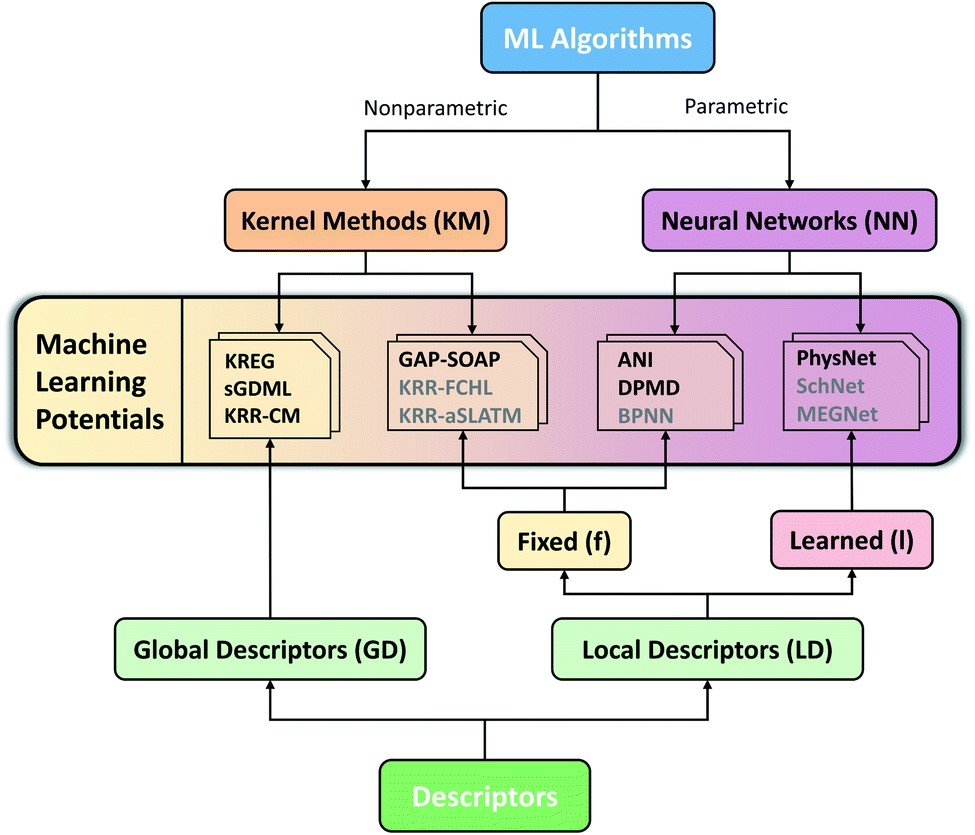
\includegraphics[width=0.7\linewidth]{figures/ML_potential_Pinheiro2021.jpeg}
\caption{Classification of frequently used ML regressors and descriptors reproduced from ref. \cite{RN39} under CC-BY 3.0.}
\label{fig:potentials}
% \figdata{This is a description of a data source.}
\end{figure*}

\subsubsection{Kernel methods}
\label{sec:kernel}
KMs use the Kernel trick, allowing linear regression algorithms to fit nonlinear functions by implicitly transforming the input data into a higher-dimensional space \cite{RN38}. KRR is straightforward and popular in quantum chemistry \cite{RN123, RN37}. KMs represent a category of simple ML methods that are relatively simple to implement from scratch; there are readily available frameworks and libraries. For instance, the scikit-learn Python library can train an arbitrary kernel method within just a few lines of code \cite{RN148}. Model performance depends on the selection of the molecular representation, that is, how we input the molecular structure to the ML model as described later. Therefore, it might be advantageous to use one of the packages developed especially for chemical applications with several representations readily available, such as MLatom \cite{RN123, RN151, RN122}, GAP \cite{RN35, RN34}, or QML code \cite{RN36}. A special kernel-based method called symmetric gradient-domain machine learning (sGDML) was also designed especially for molecular dynamics \cite{RN109, RN153, Chmiela2023}. Note that none of these codes were designed primarily for excited-state dynamics. That means that they do not natively support the fitting of the couplings. However, it can still be done \cite{RN102}. Moreover, the couplings are not always necessary to run a nonadiabatic dynamics simulation, as discussed above.

One must select a kernel (i.e., a similarity function between different geometries). Within the KRR method, the properties of interest are modeled as a linear combination of the kernel functions between the geometry of interest and the training points:
\begin{equation}
f(x) = \sum_{i=1}^{N_\text{train}} \alpha_i k(x, x_i)
\end{equation}
While the regression coefficients are set during the training procedure, the kernel has to be predefined. The two most common choices are the Laplace and the Gaussian kernel. A Gaussian kernel is usually a better choice when learning in the configuration space:
\begin{equation}
k(x, x_i) = \exp\left(-\frac{1}{2\sigma^2} \| x-x_i \|_2^2\right)
\end{equation}

\subsubsection{Neural networks}
\label{sec:nn}
The fundamental unit of an artificial NN is a single neuron, which can process simple data. The neural units are connected in layers, linked through trainable parameters. A NN typically consists of an input layer, one or more hidden layers, and an output layer. The interconnected node architecture is thus analogous to the brain; each connection has adjustable parameters that allow the network to learn from prior information \cite{RN119, RN155}.

Various packages are readily available to learn chemical properties (e.g., ground state energies) with NNs. Users need not develop the ML codebase to train and predict properties. SchNetPack \cite{RN114} is a prominent example, which includes several models like SchNet,\cite{RN136} PaiNN \cite{Schutt21}, SchNOrb \cite{RN92}, or FieldSchNet \cite{RN146}, the latter allowing the treatment of electric fields and thus environmental effects. SchNetPack offers a variety of ground state properties to predict out of the box (e.g., energy, forces, dipole moments). The default settings of these models suffice for most tasks, but significant additional parameters enable more complex tasks. 

ML photodynamics is enabled with only a few software packages. SchNarc \cite{RN103, RN142} is based on SchNetPack 1.0; it performs surface-hopping dynamics with SHARC \cite{RN139}. SchNarc predicts properties for multiple singlet or triplet states, transition dipole moments, and SOCs. Since SchNarc is based on SchNetPack 1.0, it can only be used with the invariant SchNet model, which is not problematic for scalar properties. Vectorial properties like NACs and transition dipole moments are predicted using physical relations, respectively (i.e., predicted as derivatives of virtual properties and using the charge model) \cite{RN147}. Another package that includes NNs for excited state properties is Python Rapid Artificial Intelligence Ab Initio Molecular Dynamics (PyRAI$^2$MD) \cite{RN121}. PyRAI$^2$MD has enabled mechanistic understanding of complex photochemical organic transformations such as electrocyclizations, cis-trans isomerizations, and cycloadditions \cite{RN140, RN46}.

\subsection{Molecular representations}
\label{sec:repre}

Most ML models for excited states learn the relationship between the molecular structure and their excited-state properties. In TSH trajectories, the molecular structures are represented by the Cartesian coordinates of their nuclear positions. The Cartesian coordinates are not uniquely defined as they depend on the user’s choices on the original position and orientation of the molecules in Euclidean space. As such, Cartesian coordinates must be transformed into a machine-learnable representation to satisfy the translational and rotational invariance \cite{RN136, RN33}. Classification of different descriptors that are often used in ML for chemical applications is found in Figure \ref{fig:potentials} \cite{RN39}.

\subsubsection{Representations: Application to kernel methods}
\label{sec:kernelrep}
The input feature vector representing the molecular structure is a key consideration when working with KMs. This representation should possess basic invariances. For example, molecular translations and rotations should be energy-invariant, and the representation needs to capture this truth. The representation should also be invariant to the permutation of atoms. Enforcing permutational invariance of the representation by standard techniques (e.g., atomic sorting) can lead to discontinuities in the model \cite{RN32}. Therefore, permutationally invariant kernels are desirable \cite{RN149, RN31}.

Molecular representations can be global or a set of atoms represented by local environments. Representation development has focused on local representations for ground-state applications. Some of the popular state-of-the-art local representations are the smooth overlap of atomic positions (SOAP) \cite{RN156}, atom-centered symmetry functions (ACSF) \cite{RN30}, Faber–Christensen–Huang–Lilienfeld (FCHL) representations \cite{RN29}, and others. The most common and straightforward global representations are the Coulomb matrix (CM), bag of bonds (BoB) \cite{RN137}, or normalized inverse interatomic distances (RE descriptor) \cite{RN149}. CM and RE are based on the inverse interatomic distance matrix. While these simple representations often work very well for small rigid systems, they are not permutationally invariant. BoB is based on the sorting of CM elements. While it has been shown to improve the performance in the chemical space, it has limited utility in configuration space. 

\subsubsection{Neural network representations}
\label{sec:nnrep}
The representation of the molecular structure can be handled as fixed or learned during training with NNs. Additional hyperparameters must be optimized through a thorough hyperparameter search for fixed representations and require modest computational resources. The number of requisite hyperparameters is lower for learned representation, but training is more expensive. The training process refines the representation and requires additional computational resources for the model to learn this data pattern. Thus, the choice between fixed and learned representations depends on the task's requirements, available resources, and requisite model complexity \cite{RN98}.

\subsubsection{Autoencoders}

One can generate functional descriptors automatically via a separate NN called an autoencoder \cite{RN145}. Autoencoders are NNs used for efficient data encoding, which optimizes the output of the NN to be the same as the input. However, a narrow hidden layer is used as a reduced representation after the training. Representations obtained from an autoencoder have advantages, including smaller size or differentiability when adequately designed. 

\subsection{Model training and evaluation}
\label{sec:modeltrain}
Fitting of excited state properties poses additional challenges besides fitting ground-state properties. More properties and states must be learned by ML models, and the arbitrary phase factor has to be considered. The arbitrary phase factor makes coupling between different electronic states non-unique, implying an arbitrary sign; the arbitrary sign must be corrected before or during training. A recent review discusses best practices in ML for chemistry and is recommended to consider before beginning the study \cite{RN28}.

Fitting couplings can be done by choosing an initial structure as a reference and correcting the phase for all other structures \cite{RN132}. This procedure requires computing overlap matrices between the initial structure and any other structure in the training set. Substantial overlap (>0.5 for each electronic state) can identify whether phase change has occurred by assessing the sign of the overlap. Negative overlap values suggest that a phase change has occurred; the property of the new structure must be multiplied by –1 for the given state. The same procedure must be carried out for the other state (i.e., any property has to be multiplied by –1 or +1 twice) because couplings are related to two electronic states. When the differences between two molecular structures are significant, the overlap could be too small to determine the phase factor. In this case, geometry interpolation between the two structures must be done to determine the correct phase \cite{RN132}.

Pre-processing of photodynamics data is typically cumbersome; accounting for the phase factor during training is advised. Therefore, a phaseless loss function was introduced to learn the phase factors during the training of NNs, where preprocessing NAC data does not require phase corrections \cite{RN103}. The phaseless loss function automatically multiplies the coupling data by a factor (i.e., +1 or –1) to evaluate the prediction errors. Combining phase factors with the lowest fitting error corresponds to the phase-corrected coupling data and will be used to train NNs. The main drawback of this approach is that the loss function calculations scale with $2^{N-1}$ for $N$ states. A recently developed methodology by Richardson et al. \cite{RN41} can also deal with double-valued properties.

Another challenge when learning NACs is that they are sensitive to the inverse of the energy gaps between the two electronic states $i$ and $j$ \cite{Domcke2004}:
\begin{equation}
\label{eq:NAC}
    d_{i,j} = \left< \Psi_i \left| \frac{\partial }{\partial \mathbf{R}} \right| \Psi_j\right> = \frac{\left< \Psi_i \left| \frac{\partial \hat{H}_\text{el}}{\partial \mathbf{R}} \right| \Psi_j\right>}{E_i - E_j}
\end{equation}
The magnitudes of NACs remain near zero for most regions on the excited-state PESs (see Figure \ref{fig:couplings}), except for near conical intersections or avoided crossings, where the magnitudes rapidly reach infinity as the energy gap becomes a singularity. The discontinuity of the NACs at crossing regions leads to a challenging ML task that still needs further development. A remedy to this problem is learning the numerator terms of the NACs, a continuous function of reaction coordinates avoiding cusp data \cite{RN132}. Then, the full NACs are computed on the fly by dividing the gaps between the ML-predicted energies.

The preprocessing of SOC data depends on the representations of the spin wave functions in TSH dynamics. Most QM programs compute SOCs in the spin-diabatic representation, where each spin component's SOCs between the singlet and triplet state are calculated. Due to the small SOCs (e.g., <100 cm–1) in organic molecules, the PESs are less affected by the SOCs. Thus, the norm of the SOCs can be directly used to determine the surface hopping probability at intersystem crossing regions. SOCs are known to substantially increase in molecules with heavy atoms (e.g., Br),124 it introduces important off-diagonal elements in the electronic Hamiltonian, significantly altering the topology of PESs near the intersystem crossing points. Therefore, we must diagonalize the electronic Hamiltonian with SOCs to obtain PESs in a spin-adiabatic representation. It should be noted that the SOCs lift the degenerate triplet states into different spin states (z=0, ±1) in spin-adiabatic representation, which expands the total number of states, including all spin components of a multiplet state.

Learning SOCs in the spin-diabatic representation only needs to compute the norm of SOCs without additional preprocessing. The spin-diabatic SOCs can be fitted as scalar values, similar to electronic energies. However, learning SOCs in the spin-adiabatic representation requires explicit calculations of the interstate couplings between the spin-adiabatic states. Such interstate couplings have the exact nature as the NACs, where phase corrections are needed.

\subsection{Active learning}
\label{sec:activelearn}
The complexity of applying ML algorithms to photodynamics also lies in the vast configuration space that can be visited during the dynamics. Various competing processes can occur, including rare events. The predictive regression model is limited to the configurational space included during training. Learning molecular configurations outside the training set is desirable because a training set cannot include all possible configurations – especially for chemical interconversions. Fortunately, some active learning techniques have been developed. Active learning involves calculating the ab initio properties outside the training domain, followed by regular model retraining \cite{RN155}. To that end, the user must assess the predictive variance. Some methods, such as Gaussian processes, provide predictive variances automatically, while model ensembles are implemented for other regressive models (i.e., NNs) \cite{RN131, RN105}.

The concept of active learning is shown in Figure \ref{fig:activelearning}. Panel a shows the concept of active learning. During NAMD, properties are predicted with more than one ML model or KMs and the uncertainty is estimated. In case the uncertainty exceeds a certain threshold, predefined by the user, the data point is recomputed with the reference method, added to the data set, models are retrained, and the procedure is carried on. Panel b) illustrates how the regions of the PESs are gradually covered in the training set. The arrows represent different active learning steps.

\begin{figure}[hbt!]
\begin{subfigure}{\linewidth}
\caption{}
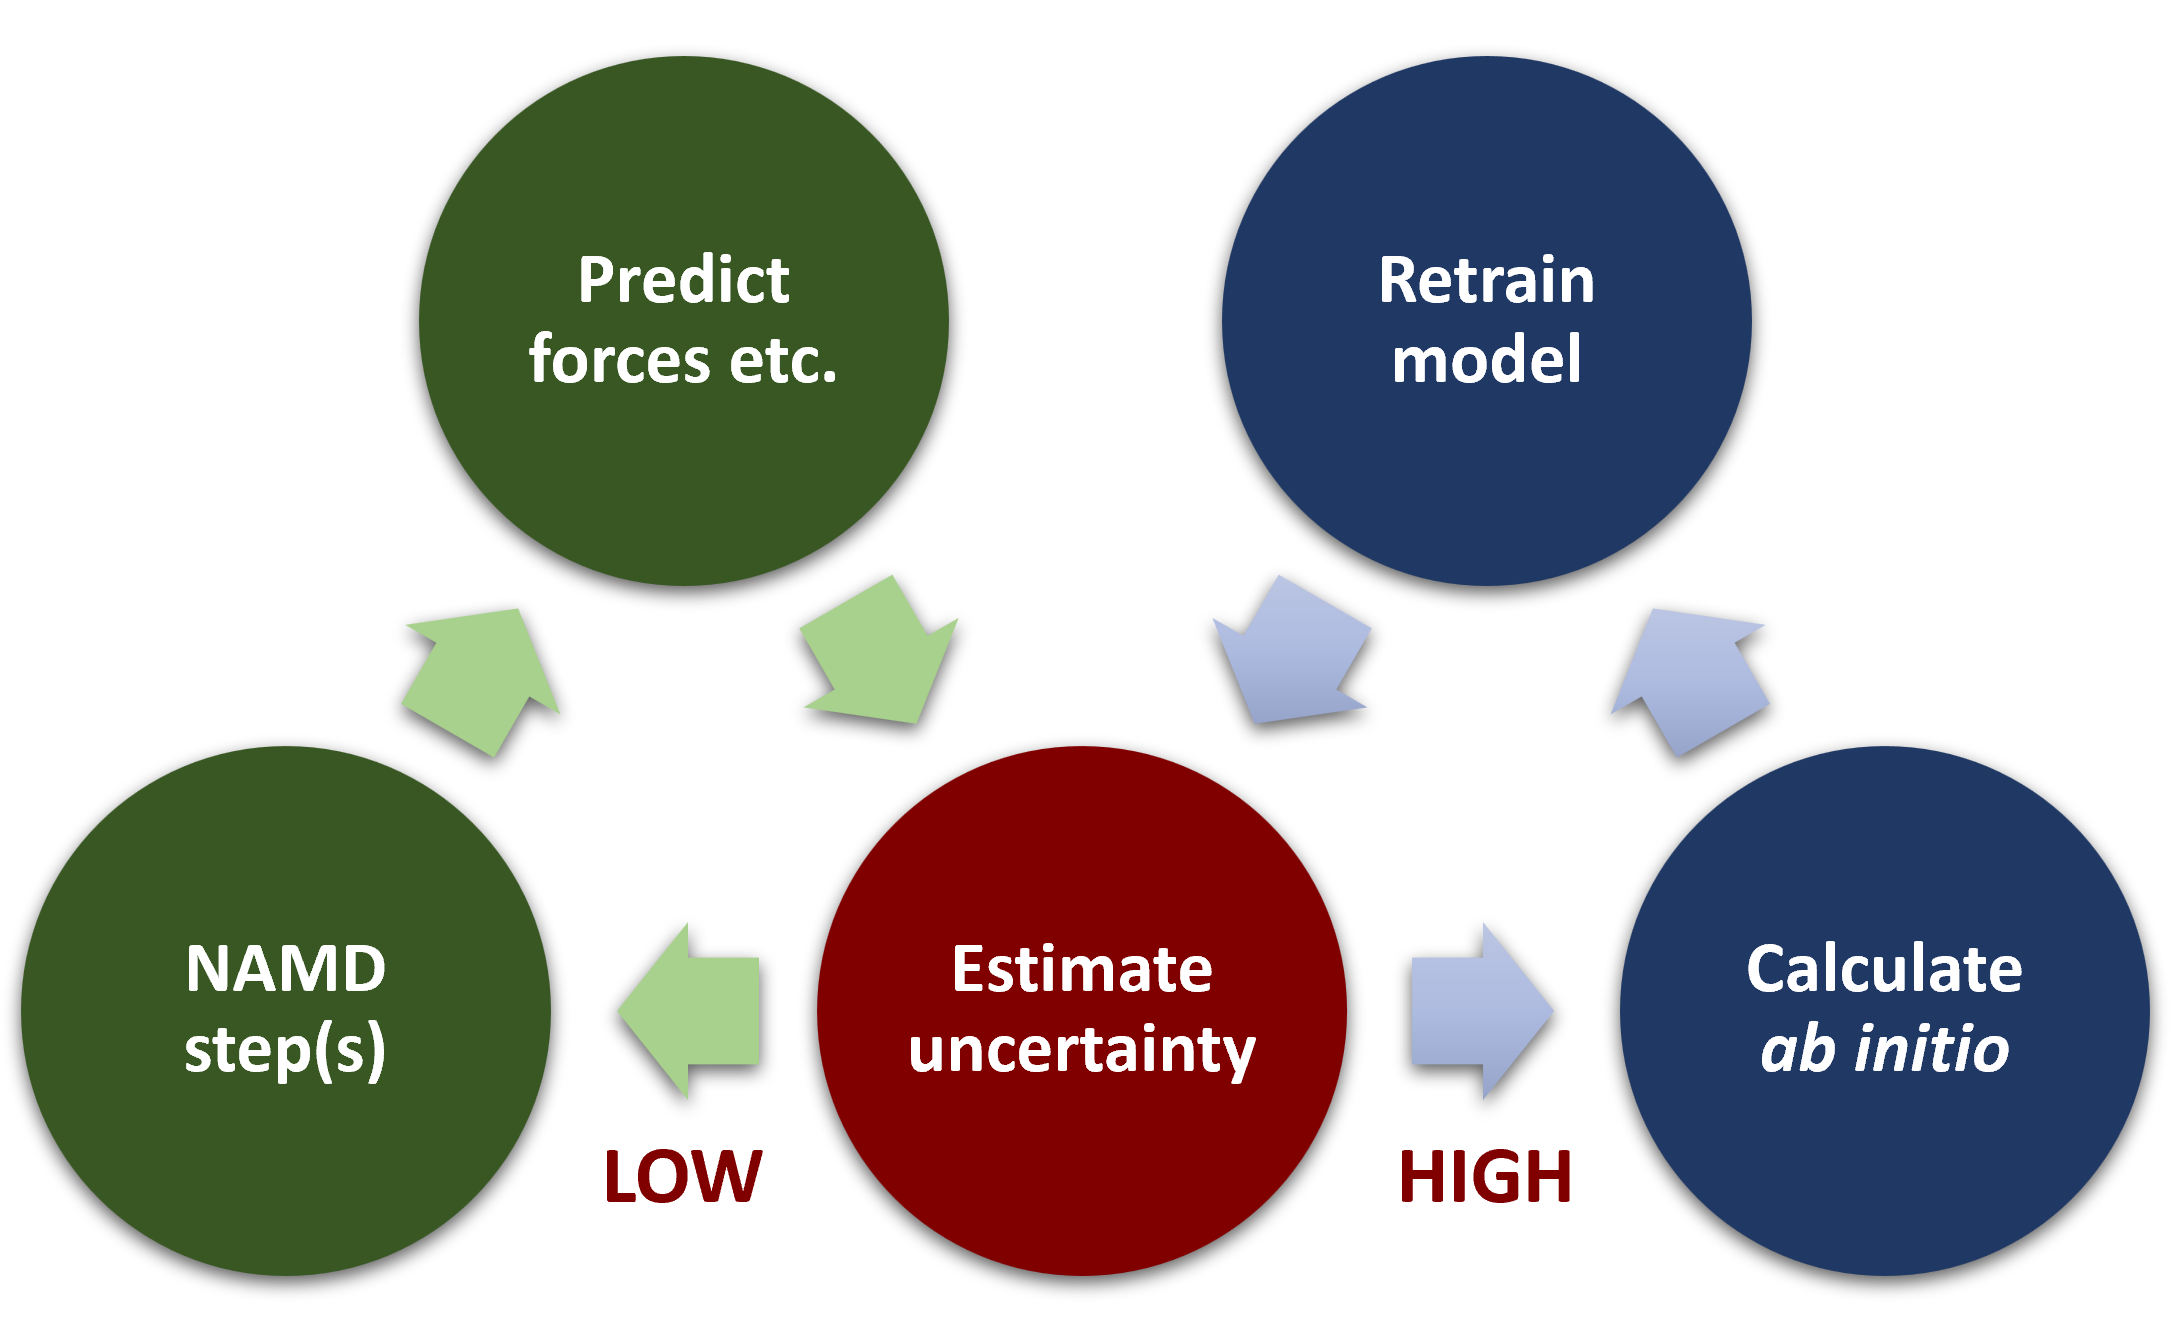
\includegraphics[width=\linewidth]{figures/active_learning1.png}
\end{subfigure}
\begin{subfigure}{\linewidth}
\centering
\caption{}
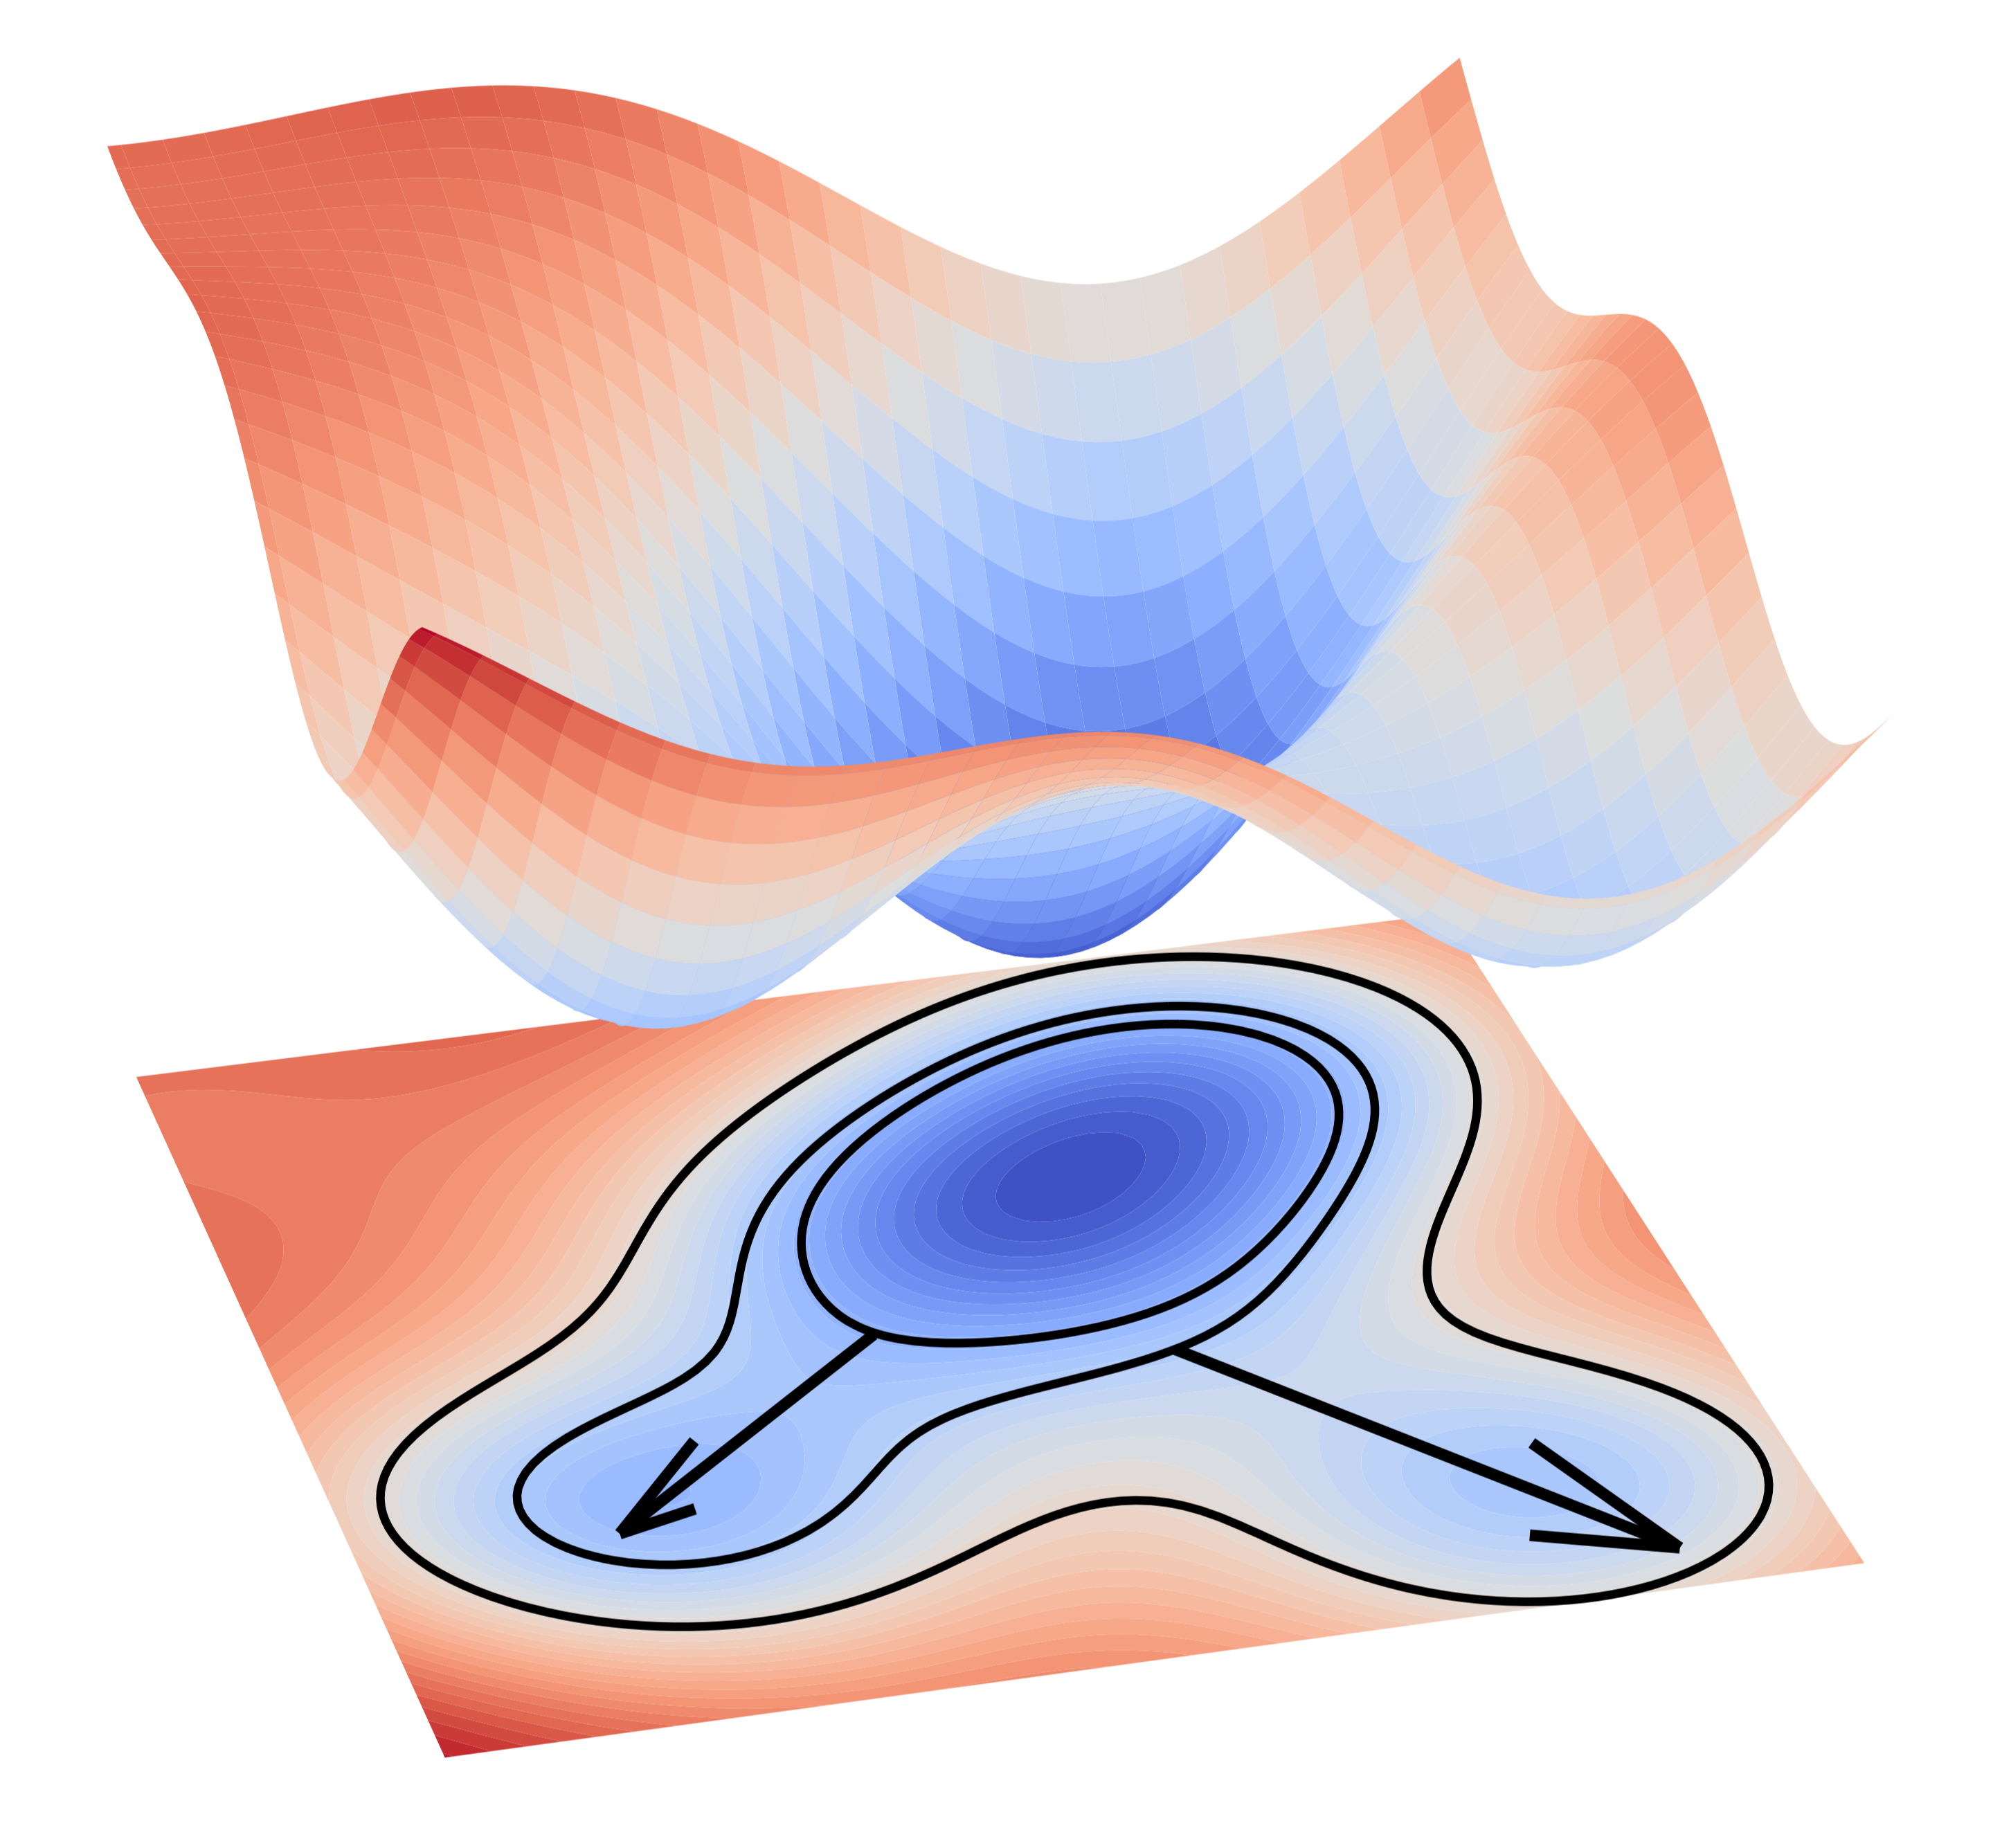
\includegraphics[width=0.8\linewidth]{figures/active_learning2.png}
\end{subfigure}
\caption{a) Simplified diagram of active learning procedure. b) Gradual expansion of the training domain with active learning when exploring a potential energy surface with molecular dynamics. Each of the arrows represents one active learning step.}
\label{fig:activelearning}
% \figdata{This is a description of a data source.}
\end{figure}

\subsection{Transferability}
\label{sec:transferability}
A user would ideally use one pre-trained ML model for accurate NAMD of another chromophore. While ML architectures are generally transferable, current ML models lack the transferability of excited states across chemical compound space, meaning a new model must be trained for each system to be investigated. Only a few approaches have been able to learn excited states of multiple systems and multiple conformations thereof, such as for UV/Vis absorption spectra \cite{RN106} or NAMD \cite{RN100}.

The transferability of pre-trained models throughout the chemical compound space represents a major problem for ML applications to excited-state dynamics. While classical force fields were used for ground-state dynamics long before the introduction of ML potentials, the same does not apply to excited states. Global representations are more efficient for the properties used in NAMD, but such models are less transferable throughout the chemical compound space than local descriptors. Even state-of-the-art studies struggle to obtain accurate predictions even when training ML models specifically for one system \cite{RN105}.

\subsection{Diabatization}
\label{sec:diabatization}

Electronic states and corresponding energies, usually from electronic structure codes, are in the so-called adiabatic representation. These are ordered by energy, and two states of the same multiplicity and symmetry never cross. Instead, they form a conical intersection, a seam of degenerate geometries. The dimensionality of such a seam is smaller by two than the system's dimensionality in internal coordinates. For example, the seam consists of just one point for a 2D system, as plotted in Figure \ref{fig:CI}.

\begin{figure}[hbt!]
\centering
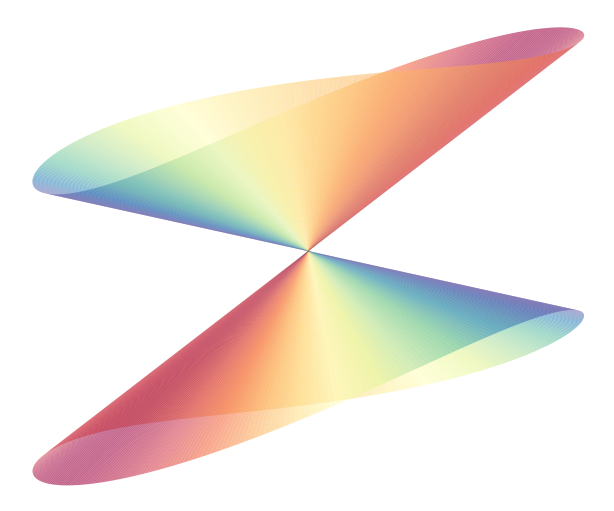
\includegraphics[width=0.7\linewidth]{figures/CI.png}
\caption{Schematic illustration of a conical intersection for a two-dimensional system. The seam of the conical intersection consists of only one point. This point separates two adiabatic states from each other while the colors represent diabatic characters.}
\label{fig:CI}
% \figdata{This is a description of a data source.}
\end{figure}
 
Conical intersections are incredibly challenging for surface fitting because of the discontinuous potentials near the seam. And, of course, NACs are singular at conical intersections. It is thus advantageous for potential fitting to switch to a different basis to enable smooth evolution along geometrical coordinates with a geometry-dependent transformation matrix $\mathbf{T}(\mathbf{R})$:
\begin{equation}
\Psi_i^\text{diab} (\mathbf{r};\mathbf{R}) = \sum_j^{N_\text{states}} T_{ji}(\mathbf{R}) \Psi_j^\text{adiab} (\mathbf{r};\mathbf{R})    
\end{equation}
The corresponding potential energy matrix is given by the following transformation of the diagonal matrix of adiabatic energies:
\begin{equation}
\mathbf{U}(\mathbf{R}) = \mathbf{T}^\text{T}(\mathbf{R}) \mathbf{V}(\mathbf{R})\mathbf{T}(\mathbf{R})    
\end{equation}
Note that the resulting matrix of energies is no longer diagonal; the off-diagonal elements (diabatic couplings) must also be fitted.
The basis in which the NACs vanish completely is called a diabatic basis. Unfortunately, such a basis does not generally exist for molecules with three or more atoms \cite{Mead1982ConditionsSystems}. Therefore, the definition of diabatic basis is ambiguous. The transformation matrix cannot be clearly defined, and many different approaches have been proposed \cite{RN26}. On the other hand, the reverse transformation from a diabatic to an adiabatic basis can be achieved by diagonalization. Other properties apart from energies can also be predicted in the diabatic basis. While atomic forces and approximate NACs can be directly obtained from the diabatic representation, other properties can be fitted separately using the calculated transformation matrix \cite{RN25, RN24}.

The diabatic basis is convenient for ML because of its smoothness. However, diabatization is an outstanding problem itself, and multiple approaches exist. The diabatization already requires expert knowledge about the system; see the review by Shu et al. for a detailed discussion \cite{RN26}. The recommendation is to switch to a diabatic basis whenever possible for a given system. Even for surface hopping, which has been shown to work better on the adiabatic basis \cite{RN154, RN139}, the ML training can be performed in the diabatic basis and diagonalized to reform the adiabatic basis.

Even though it is so convenient, obtaining a diabatic representation is usually difficult so this task is often left to cases where quantum dynamics is needed. The fitting of adiabatic energies and properties for TSH has proved to be feasible, barring non-smooth cusps. The dynamics are reliable because hopping events occur near conical intersections but not exactly on the seam. This simplifies the problem because the exact seam is not reproduced as accurately as the rest of the potentials. 

\section{Post-processing}
\label{sec:postprocessing}

ML-driven excited-state molecular dynamics have revolutionized photochemistry by enabling the simulation of thousands of trajectories over nanosecond timescales. Consequently, the analysis of the resulting data has transformed into a big data problem, surpassing the capabilities of traditional visual inspection and trajectory analysis methods. Novel techniques are required to comprehensively analyze the data and extract pertinent information. We describe best practices for investigating ML- and QM nonadiabatic trajectories, incorporating various recent approaches in the literature. To illustrate these techniques, we will present examples involving the analysis of TSH dynamics data for the methylenimmonium cation \cite{RN132}.

The section will be divided into four parts: prior considerations, dimensionality reduction, and clustering analyses of static data, which involves analyzing all the data simultaneously, considering each point individually, and dynamic analysis, which focuses on analyzing data as a time series. We will not delve into the analysis of individual trajectories, as comparisons to experimental data necessitate the examination of statistical averages rather than individual events. 

An example jupyter notebook for the analysis of trajectory data from excited-state calculations can be found at the following link: \url{https://colab.research.google.com/drive/14W3zqhvSjHxUkSM_JrSbQiU_G6cSBmQK?usp=sharing}. 

\subsection{Prerequisites and preparative considerations}
\label{sec:preparepostprocess}
Before diving into the details of excited-state trajectory data analysis using ML-based techniques, we want to highlight the importance of the data quality. Especially if the NAMD is based on ML potentials, the trajectories might sometimes be error-prone. We urge users to search for undefined or missing values and outliers. For example, if an NVE ensemble is used, the user should check for validating constant total energy during each trajectory simulation. 
 
The choice of features included, and the representation are crucial for the outcome of any ML method, as already emphasized in section \ref{sec:repre}. For postprocessing analyses, this depends on – and is limited by – the NAMD data aspects, the research question, and the extent of knowledge about the chemical problem. Many possible representations exist for geometrical information. However, to maintain interpretability, intuitive representations and features are chosen, such as the pairwise distances \cite{RN23}, any combination of interatomic distances, angles, and dihedrals \cite{RN22}, based on the pairwise dissimilarity matrix between two configurations \cite{RN21}, or as normal mode coordinates representations \cite{RN144, Hase2020}.

The data should be normalized or scaled to avoid biases from different descriptors. The possibilities depend on the nature of the data and include a mere shift of the mean to zero, min-max normalization (subtraction of the minimum followed by dividing by the maximum-minimum difference), z-score scaling (subtraction of mean followed by division by standard deviation), and the division by the respective quantities of a reference data point (e.g., global minimum structure).

\subsection{Dimensionality reduction}
\label{sec:dimred}

Molecular data is complex because of the substantial number of degrees of freedom; it cannot be easily represented in one or two dimensions for visualization. Reducing the data's dimensionality becomes crucial while retaining its fundamental structure. Dimensionality reduction techniques are invaluable in such scenarios because they address the challenges posed by the high dimensional data and aid in visualization, exploration, and interpretation.

Principal Component Analysis (PCA) is one of the most widely used linear dimensionality reduction methods. It transforms the original high-dimensional data into a lower-dimensional space by identifying the directions of maximum variance in the data. The obtained set of uncorrelated variables is known as the principal components. The input to PCA is standardized descriptors that are pre-defined geometric and or property-based quantities that represent the molecular system under investigation. The covariance matrix of the input features is computed to capture the correlation between the variables. This matrix is decomposed into its eigenvectors and eigenvalues, where the eigenvectors with the largest eigenvalues correspond to the principal components containing most of the data's variance. These principal components determine the new coordinate system for the transformed data. The first few main components will ideally include most of the variance in the data, enabling dimensionality reduction to visualize the data in a few dimensions. This is most effective on jointly Gaussian-distributed data because no correlation between components implies independence \cite{RN20}. 

PCA enables the interpretation of the transformed features by investigating how much each pre-defined descriptor contributes to each principal component, revealing the relative importance of each feature. Kernel PCA is an extension of PCA that allows for nonlinear dimensionality reduction. It uses a kernel trick technique to implicitly map the data into a higher-dimensional feature space, where linear PCA is performed. By utilizing a nonlinear mapping, kernel PCA can capture more complex and nonlinear patterns in the data \cite{RN11}.

Multidimensional scaling (MDS) is another common category of nonlinear dimensionality reduction methods, especially useful for visualisation \cite{Mead1992ReviewMethods}. MDS encompasses several algorithms reconstructing a low-dimensional spatial representation while preserving given pairwise distances or dissimilarities among data. Unlike other methods, MDS can handle any dissimilarity measure, making it applicable to a broad range of data types in chemistry, such as bond distances, angles, or torsional angles. The primary goal of MDS is to create a map with coordinates in a lower-dimensional space (usually 2 or 3 dimensions) that reflects the pairwise dissimilarities among the data points. These coordinates place each data point in the new space in such a way that the Euclidean distance between them closely matches the original dissimilarity measure.

The algorithms most frequently applied are classical MDS, metric MDS, and non-metric MDS. Classical MDS is particularly useful when the original dissimilarities are based on metric measurements, such as bond lengths or angles. Metric MDS is designed to handle metric dissimilarities explicitly, ensuring that the distances in the reconstructed map satisfy the properties of a metric space. It is a valuable approach when the dissimilarity measure is derived from real distances with a consistent scale. Non-metric MDS can accommodate non-metric dissimilarities, which may not satisfy the triangle inequality. Non-metric MDS is often employed when direct metric measurements are unavailable and only ordinal relationships between molecules are known \cite{RN14}.

Another nonlinear dimensionality reduction technique is isomap, which focuses on preserving the intrinsic geometry and manifold structure of the data. It leverages the concept of geodesic distances, measuring the shortest path along the manifold between data points. The critical steps in isomap include the construction of neighborhood graphs, computing the geodesic distances between data points connected via the neighborhood graph, and embedding the data into a lower-dimensional space. The latter transformation uses MDS to preserve the geodesic distances as much as possible. Isomap is particularly useful for datasets with nontrivial geometric or topological properties that are difficult to analyze with linear methods.\cite{RN94, RN12}

Other popular nonlinear dimensionality reduction techniques are t-SNE (t-Distributed Stochastic Neighbor Embedding) and UMAP (Uniform Manifold Approximation and Projection).  t-SNE captures local structure and similarities between data points by constructing a probability distribution in the high-dimensional space, thus representing pairwise similarities between data points and a corresponding distribution in the low-dimensional space. It is especially effective at preserving local structures, enabling cluster visualization for identifying patterns within complex molecular datasets \cite{RN10}.

UMAP is another nonlinear technique that focuses on preserving the global structure and connectivity of the data. It constructs a high-dimensional topological representation of the data and then optimizes a low-dimensional representation that preserves the topological relationships. UMAP is based on manifold learning and is particularly useful for capturing local and global structures in high-dimensional data. It can handle large datasets more efficiently than t-SNE while producing similar embedding results \cite{RN20}.

\subsection{Pattern recognition and point-based data clustering}
\label{sec:clustering}

Pattern recognition encompasses a broad array of tools designed to identify patterns within data and group them accordingly. These tools can be categorized into clustering and classification methods. Classification techniques are part of supervised learning, where labeled data is available, allowing data points to be assigned to predefined classes. In contrast, clustering techniques belong to unsupervised learning, where data points are grouped into clusters based on their inherent similarities. The key distinction lies in the presence or absence of labels, making unsupervised learning approaches, particularly clustering, well-suited for analyzing molecular dynamics simulations where labels are typically unavailable. Labeling data before analysis is often impractical with large and complex datasets. Consequently, unsupervised techniques offer a more straightforward starting point for analyzing and exploring patterns within dynamic data, making them the primary focus of this section. Clustering algorithms uncover hidden patterns and structures within datasets \cite{RN20}. 

\subsubsection{Selecting a proper clustering algorithm}

The nature of the data, the desired outcome, and the specific problem factors should be considered when choosing a clustering method. We advise gaining a basic understanding of the data. This understanding can be obtained by examining the data's dimensionality, the flexibility of the system, and any assumptions about the expected processes found in the literature. Once some understanding of the data is established, the objective of the clustering analysis needs to be defined. We suggest considering the following questions: Are you aiming to identify outliers? Is the primary goal to reduce the data dimensionality? Do you try to discover natural groups representing structures near mechanistic critical points on potential energy surfaces or photoproducts? 
Different clustering techniques may be selected depending on the case. We suggest comparing various clustering algorithms to make an informed decision. If the dataset is too large, using a randomly generated subset can be beneficial for comparing different algorithms \cite{RN97, RN135, RN130}.

K-means clustering partitions the data into a predefined number of clusters (K) by minimizing the within-cluster sum of squares. K-means clustering requires a distance metric and is suitable for continuous variables. It assumes clusters of similar sizes and spherical shapes \cite{RN19}.

Hierarchical clustering, as the name implies, creates a hierarchical structure of clusters by merging or splitting clusters based on their similarity or dissimilarity. It does not require prior specification of the number of clusters and can handle both continuous and categorical variables.\cite{RN148} 

Density-Based Spatial Clustering of Applications with Noise (DBSCAN) identifies clusters based on regions of high density separated by regions of low density. It is suitable for data with irregularly shaped clusters and effectively handles noise and outliers \cite{RN96}.

Gaussian Mixture Models (GMM) are useful when the number of clusters is difficult to determine. While it starts with an initial guess of the number of clusters, it provides suggestions for a suitable number. GMM assumes that the data points are generated from a mixture of Gaussian distributions. It can estimate the distribution parameters and assign probabilities to data points belonging to each cluster \cite{RN18}.

We recommend exploring the scikit-learn library for more clustering techniques, which provides a comprehensive overview of different clustering methods and their use cases \cite{RN148}. Note that experimenting with various methods of clustering or parameter settings can be highly valuable because there is usually no general solution. Still, many processes might lead to similar results or can provide complementary information. Selecting a clustering method may require iterative refinement based on the data's specific characteristics and the desired outcome. 

\subsubsection{Evaluating the performance of clustering}

Assessing the performance of clustering algorithms presents distinct challenges due to the absence of labeled data in unsupervised learning and, thus, the absence of a metric to evaluate the performance. This paper explores various extrinsic and intrinsic evaluation measures to overcome this limitation.

The distinction can be made between extrinsic and intrinsic measures. Extrinsic measures rely on externally provided labels or known class assignments to evaluate clustering performance. Thus, they are often not practicable when clustering dynamics data of which no labels are accessible before analysis. Examples of extrinsic measures are the rand index (measuring the similarity between two clusters by comparing pairs of samples), mutual information (quantifying mutual dependence between clusters), V-measure (assessing homogeneity and completeness of clusters), or Folkes-Mallows score (determining the similarity between two clusters by comparing geometric means).

More practicable for our use case are intrinsic measures that assess clustering quality based solely on the characteristics of the clustering itself and the underlying data without requiring any external labels. They thus aim to capture how well the data points within each cluster are grouped and how distinct the clusters are from one another. Intrinsic measures include the Silhouette Coefficient, Calinski-Harabasz Index, and Davies-Bouldin Index.

The Silhouette Coefficient or Silhouette Score evaluates the performance based on the distance of data points within clusters $a$ (average intra-cluster distance) and the distance of different clusters $b$ (average inter-cluster distance) \cite{ROUSSEEUW198753}:
\begin{equation}
\label{eq:silhouette}
\text{Silhouette score} =  \frac{b-a}{\max(a,b)}
\end{equation}
The silhouette score ranges from -1 to 1, where 1 means that clusters are well separated, 0 means no significant distance between clusters, and -1 implies that clusters are not assigned correctly.

The Calinski-Harabasz index uses the ratio of between-cluster variance to within-cluster variance. The higher the index, the better the clusters are defined. The Davies-Bouldin score measures the average similarity of a cluster with respect to its most similar cluster. Lower values indicate better clustering performance \cite{RN148, RN17}.

\subsubsection{Cluster visualization and data extraction}

After executing and evaluating the clustering, visualizing the results is needed to extract chemical insights. One common approach involves a scatter plot; two or three descriptors are used to plot the data in the feature space. The inputs to the scatter plot are features known to be important for the reaction under investigation, or high-dimensional inputs already transformed into lower-dimensional representation with dimensionality reduction techniques, as discussed in section \ref{sec:dimred}. Using colors, shapes, or markers to indicate the different clusters while plotting the data is useful. Scatter plots allow for an overview of the distribution and separation of clusters in the feature space. MDS is a very common technique to plot a low-dimensional representation of high-dimensional data. t-SNE and UMAP are also frequently applied to visualize high-dimensional molecular data as these methods aim to preserve the local structure of the data and reveal clusters and patterns in the molecular dataset.

Exploring molecular interactions and connectivity patterns can be achieved with network visualization techniques such as Cytoscape \cite{RN16}. Molecular data are represented as a network or graph, where molecules are nodes, and their relationships are edges. Clusters can be visualized as subgraphs or communities within the larger network.

Besides these visualization techniques, additionally inspecting the clusters visually is often inevitable. Therefore, cluster centroids can be computed and serve as representatives of each cluster, reducing the complexity and time required for the visual inspection \cite{RN104, RN148}.

\subsection{Time series clustering}
\label{sec:timeclustering}

Analyzing molecular dynamics data with time series techniques can provide valuable insights into the system's dynamic behavior. Some of the most useful time series techniques include descriptive statistics, time plots, autocorrelation, and partial autocorrelation analysis. Descriptive statistics can help characterize the behavior of molecular properties over time. Calculating statistics such as mean, standard deviation, or autocorrelation of molecular properties (e.g., bond lengths, angles, dihedral angles) can provide insights into their stability, fluctuations, and correlations.

Time plots are probably the most intuitive approach because they demonstrate how molecular properties evolve throughout the simulation. Plotting molecular properties against time allows for identifying trends, fluctuations, and potential patterns or events in the system. Autocorrelation analysis can reveal the presence of correlations or dependencies in molecular data over different time lags. It helps identify any time-dependent patterns or autocorrelated behavior within the system. Fourier Transform applied to molecular dynamics data can identify dominant frequencies or periodicities in molecular motions. It helps uncover characteristic vibrational modes, collective motions, or oscillatory behavior within the system.

Tslearn is a Python library designed for time series analysis \cite{RN13}. It provides many tools and algorithms for analyzing, modeling, and visualizing time series data. Some of the key features and techniques offered by tslearn include time series clustering and time series classification, which enable clustering and classification of time series into predefined classes or categories, respectively, time series forecasting, or time series distance metrics to allow for quantification of similarities and dissimilarities between time series sequences.


\clearpage

%Here we use a full-page checklist with multiple sections, so it will appear on a separate page of the sample PDF.
%Other checklist formats are possible, as shown in the sample \texttt{sample-document.tex} in \url{github.com/livecomsjournal/article_templates/templates}.

%Your checklist should include a succinct list of steps that people should follow when carrying out the task in question.
%This is provided to ensure certain basic standards are followed and common but critical major errors are avoided.
%Note that a checklist is not intended to cover \emph{all} important steps, but rather focus on the most common reasons for failure or incorrect results, or issues which are particularly crucial.


% This provides a checklist which
% - spans a full page
% - consists of multiple sub-checklists
% - exists on a separate page
% This style of checklist will be especially helpful if you want to encourage readers to print and use your checklist in practice, as they
% can easily print it without also printing other material from your manuscript. However, other styles of checklist are also possible (below).

\begin{Checklists*}[p!]
\section{Checklists}

\begin{checklist}{Pre-processing}
\begin{itemize}
\item Confirm the suitability of machine learning potentials before starting --- does the project at hand require extensive nonadiabatic dynamics simulation?
\end{itemize}

\textbf{Selection of the NAMD algorithm and electronic structure method}
\begin{itemize}
\item Ensure sufficient accuracy of the method (\textit{e.g.} in comparison to experimental data).
\item Ensure suitability for the chemical system at hand.
\item Note that the NAMD algorithm largely determines the quantities to be learned (e.g. TSH methods might require NACs or SOCs in addition to energies and forces (Section~\ref{sec:surfacehop})).
Thus, ensure that the electronic structure code to be used provides all necessary quantities for the NAMD simulation.
\item Ensure viable computational cost of the electronic structure method (Section~\ref{sec:elstructure}) or alternatively, consider employing $\Delta$ML or transfer learning between chemical methods.
\end{itemize}

\textbf{Obtaining training data}
\begin{itemize}
\item For trajectory-based methods, keep in mind that the generated initial conditions have a large impact on the dynamics and thus the conformational space available for training (Section~\ref{sec:initcond}).
\item Sample a sufficient number of structures near degenerate regions beyond even sampling of trajectories (Section~\ref{sec:trajdatachoice}).
\item Do not miss any quantities. Oftentimes in TSH simulations not all, but only the required partial gradients and coupling terms are computed in each time step (Sections \ref{sec:energyandgradients} and \ref{sec:couplings}).
\item Keep in mind that an undersized initial dataset size can be extended via active learning approaches.
\end{itemize}
\end{checklist}



\begin{checklist}{Surface-fitting}
\textbf{Choice of ML model}
\begin{itemize}
\item Choose on individual basis.
\begin{itemize}
    \item Kernel methods (KRR, GPs, SVM, \dots; see Section~\ref{sec:kernel}) are more suitable for small data (<2000 data points).
    \item Neural networks (Section~\ref{sec:nn}) perform better for big data.
\end{itemize}
\item Consider the available packages.
\begin{itemize}
    \item Set up a python library or software package designed for ground state potentials to work for excited states.
    \item OR: Use one of few software packages enabling NAMD (PyRAI$^2$MD \cite{RN121}, SchNarc \cite{RN103,RN142}).
\end{itemize}
\end{itemize}

\textbf{Choice of descriptor}
\begin{itemize}
\item Note that the descriptors are limited by the model and program package chosen (Section~\ref{sec:repre}).
\item Ensure that the representation possesses basic invariances and equivariances.
\item Consider the system (size) when choosing the representation (see Section~\ref{sec:kernelrep} for global and local representations within kernel methods).
\item When opting for NNs: decide between fixed and learned representations (Section~\ref{sec:nnrep}).
\end{itemize}

\end{checklist}
\end{Checklists*}


\begin{Checklists*}[p!]
\begin{checklist}

\textbf{Additional challenges}
\begin{itemize}
\item Recognize the phase problem of the coupling terms (Section~\ref{sec:modeltrain}):%(the arbitrary phase factor of the wave function leads to arbitrary signs of coupling terms (NAC data))
\begin{itemize}
\item Correct all phases in advance with the wave function overlap technique.
\item OR: Account for the phases during training (via a phaseless loss function or double-valued properties).
\end{itemize}
\item Account for discontinuities of the potentials in the adiabatic representation (in addition to providing sufficient data points in regions with discontinuities).
\begin{itemize}
\item Consider learning in diabatic representation for smooth quantities 
(Section~\ref{sec:diabatization}).
\item Consider learning NACs multiplied with the energy gap to alleviate the energy gap sensitivity (discontinuities at crossing regions are an ongoing challenge; see Section~\ref{sec:modeltrain}).
\end{itemize}
\item Transferability of NAMD ML models is currently still limited (Section~\ref{sec:transferability}).
\end{itemize}

\textbf{Evaluation of the ML model}
\begin{itemize}
\item Always evaluate the performance of your trained model.
\item Use active learning to assure reliability when employing the ML model (Section~\ref{sec:activelearn}).
\end{itemize}
\end{checklist}



\begin{checklist}{Post-processing}
\begin{itemize}
\item Check for missing values and outliers before further processing
\item Choose features and an adequate representation for data-driven analyses.
\begin{itemize}
\item Ensure intuitive representations for better interpretability.
\item Scale the data to avoid biases, especially when using different data quantities such as atomic distances and angles (Section~\ref{sec:preparepostprocess}).
\end{itemize}
\end{itemize}
\textbf{Selection of algorithms for NAMD data analysis}
\begin{itemize}
\item Employ dimensionality reduction algorithms to obtain the most relevant features (via e.g. PCA, MDS, \dots; see Section~\ref{sec:dimred}). \\(Further note that employing such algorithms is also relevant in the context of wave function propagation methods where the cost impedes the use of full dimensionality.)
\item Use point-wise clustering schemes to identify patterns (such as frequently visited regions in phase space) (via e.g. DBSCAN, agglomerative clustering, \dots; see Section~\ref{sec:clustering}).
\item Use time-series clustering to find patterns in the dynamical behaviour and obtain typical trajectories (Section~\ref{sec:timeclustering}).
\item Visualise the outcome of the data analysis for further interpretation.
\end{itemize}
\end{checklist}

\end{Checklists*}

\clearpage
\section{Perspectives and conclusion}

\subsection{Quantum Dynamics}

Machine learning tools are being developed that help accelerate and enable the running and analysis of NAMD using trajectory-based methods such as TSH. Full quantum dynamics methods that propagate a delocalized wavepacket also stand to gain much from these techniques. However, complications resulting from their computationally intensive nature point towards slower advances in this subfield. 

Full quantum dynamics methods solve the time-dependent Schrödinger equation by propagating the complete wavepacket on a grid. The Multi-configuration Time-Dependent Hartree (MCTDH) method is an example of this approach \cite{RN87}. The surface hopping methods require accurate potential surfaces and NACs, which can be provided in principle by the techniques described in section \ref{sec:fitting} above. Gradients are not required, only energies. Unlike trajectory-based methods, however, global surfaces are needed. A diabatic representation is required (section \ref{sec:diabatization}). While the surfaces only need to be accurately described in the region of space occupied by the wavepacket, their delocalized nature means that it is sensitive to “holes” in the potential, i.e., regions where the potential drops to large negative energies due to poor fitting. A likely problem is if sufficient data is not used when learning surfaces, particularly at the boundaries of the space to be covered.

One can provide the data samples by using the surface hopping data. However, the classical nature of these trajectories may mean that they do not sample the full space needed to describe the wavepacket. Gaussian wavepacket methods, such as Multiple Spawning \cite{RN86} or vMCG \cite{RN9}, may provide the answer by collecting data along trajectories that can be related directly to the wavepacket motion. This is in particular for the case with vMCG where the trajectories are not classical and spread faster to cover the needed phase space. vMCG has been shown to provide the points for Shepard Interpolated surfaces during direct dynamics simulations \cite{RN40, RN8} and use more advanced sampling techniques in the GROW methodology \cite{RN7}. More recently, it has been used with Gaussian Process Regression to learn the potentials for MCTDH calculations \cite{RN6}. However, the latter simulations also showed the challenges as many points were required for accurate surfaces.

ML techniques can take a complicated multi-dimensional potential function and put it in the form required for efficient quantum dynamics simulations. An ongoing challenge is the high computational cost of multi-dimensional integrals; the potential must be in a “sum-of-products” form. The sum-of-products formalism is written as a sum of terms comprising low-dimensional functions multiplied together. NNs are suitable for this \cite{RN5, RN4}, but have only been applied to small systems.

More and more research is directed towards post-processing (section \ref{sec:postprocessing}). Unlike surface hopping, which gives easily visualizable results with chemical structures moving along trajectories, wavepackets have all the information in a complex multi-dimensional function. Extracting trajectories of molecules evolving in time across excited- and ground-state PESs would help to create unprecedented knowledge of molecular excited states. Sampling and clustering techniques (sections \ref{sec:clustering} and \ref{sec:timeclustering}) to find the significant regions are useful, but visualizing correlations is needed to demonstrate how wavepacket components evolve coherently.

\subsection{Final Notes}

ML for excited states is much less explored, unlike ML for ground-state molecular properties. While ML ground-state potential energy surfaces can be obtained with high accuracy, errors for fitting excited-state properties are generally higher. The benefit of ML potentials that give very low errors with respect to QM methods, as it is often discussed in ground-state simulations \cite{RN127, RN95, Schutt21, RN126, RN93}, provide record-setting timescales for NAMD simulations.

A major challenge that remains to be solved is transferability. Notably, the number and character of electronic states within a certain energy range can vary dramatically even between seemingly similar molecules.5 ML offers the possibility to carry out many hundreds of NAMD trajectories that are needed to achieve statistically significant results. Therefore, active learning techniques are often indispensable when carrying out ML-driven NAMD. In addition, the high amount of data produced by ML-driven NAMD will likely require other advanced ML-based methods for postprocessing and analysis in the future. The benefit of using equivariant features in ML for fitting potential energy surfaces and properties thereof is in its infancy. Much work is still needed to push this field forward and benchmark data sets are required to allow for developing and testing new ML methods for excited states. Efforts in the future should thus be further devoted to data set creation in addition to ML development and testing. 



\section*{Author Contributions}
%%%%%%%%%%%%%%%%
% This section must describe the actual contributions of
% author. Since this is an electronic-only journal, there is
% no length limit when you describe the authors' contributions,
% so we recommend describing what they actually did rather than
% simply categorizing them in a small number of
% predefined roles as might be done in other journals.
%
% See the policies ``Policies on Authorship'' section of https://livecoms.github.io
% for more information on deciding on authorship and author order.
%%%%%%%%%%%%%%%%

All authors contributed to the discussion that led to this manuscript and the initial draft. SAL and JW oversaw the writing of the manuscript. Individual groups formed that prepared the initial draft of each section. CM, SAL, and RCO focused on section \ref{sec:preprocessing}. SM, GW, JL, and ŠS focused on section \ref{sec:fitting}. BB, MPJ, and JW focused on section \ref{sec:postprocessing}. All authors were involved in the revision process. ŠS prepared the original figures. BB prepared the Jupyter notebook on unsupervised learning.

% We suggest you preserve this comment:
For a more detailed description of author contributions,
see the GitHub issue tracking and changelog at \githubrepository.

\section*{Other Contributions}
%%%%%%%%%%%%%%%
% You should include all people who have filed issues that were
% accepted into the paper, or that upon discussion altered what was in the paper.
% Multiple significant contributions might mean that the contributor
% should be moved to authorship at the discretion of the a
%
% See the policies ``Policies on Authorship'' section of https://livecoms.github.io for
% more information on deciding on authorship and author order.
%%%%%%%%%%%%%%%

This work is the result of the CECAM workshop "Machine-learned potentials in molecular simulation: best practices and tutorials" of July 2023 organized by Chris Oostenbrink and JW. 
The authors thank all participants for fruitful discussions. 

% We suggest you preserve this comment:
For a more detailed description of contributions from the community and others, see the GitHub issue tracking and changelog at \githubrepository.

\section*{Potentially Conflicting Interests}
%%%%%%%
%Declare any potentially competing interests, financial or otherwise
%%%%%%%

The authors declare no potential conflict of interest.

\section*{Funding Information}
%%%%%%%
% Authors should acknowledge funding sources here. Reference specific grants.
%%%%%%%
%CM gratefully acknowledges funding by the Alexander von Humboldt foundation within a Feodor Lynen fellowship. 
ŠS gratefully acknowledges the support of Czech Science Foundation, project No. 22-13489O. RCO acknowledges funding from the Leverhulme Trust Leverhulme Trust (RPG-2019-122). RCO and SAL acknowledge the Royal Society for funding through an International Exchange Grant (IES\textbackslash R2\textbackslash 222057). SAL acknowledges the National Science Foundation (NSF-CHE-2318141) for funding. MPJ acknowledges the financial support of the European Research Council (ERC) under the advanced grant SubNano (No 832237).

\section*{Author Information}
\makeorcid

\bibliography{library}

%%%%%%%%%%%%%%%%%%%%%%%%%%%%%%%%%%%%%%%%%%%%%%%%%%%%%%%%%%%%
%%% APPENDICES
%%%%%%%%%%%%%%%%%%%%%%%%%%%%%%%%%%%%%%%%%%%%%%%%%%%%%%%%%%%%

%\appendix


\end{document}
